\documentclass[a4paper]{article}
\usepackage{geometry}
\geometry{left=3.5cm,right=3.5cm,top=3.5cm,bottom=3.5cm}
\usepackage{amsmath, amssymb}
\usepackage{graphicx}
\usepackage{subfigure}
\usepackage{pdfpages}
\usepackage{multirow}

\usepackage{xeCJK}
\setmainfont{Times New Roman}
\setCJKmainfont[BoldFont=SimHei,ItalicFont=KaiTi]{SimSun}

\usepackage{indentfirst}
\setlength{\parindent}{2em}

\usepackage{fancyhdr}
\pagestyle{fancy}
\usepackage{lastpage}
\rhead{}
\lhead{}
\cfoot{\thepage{}}
\renewcommand{\headrulewidth}{0pt}
\renewcommand{\figurename}{图}
\renewcommand{\tablename}{表}
\renewcommand{\abstractname}{摘要}
\renewcommand{\contentsname}{\CJKfamily{SimHei} 目录}

\headheight 14pt

\usepackage{float}

\renewcommand\baselinestretch{1.2}

\begin{document}

%\begin{titlepage}
%\includepdf[pages=2-3,offset=0cm 0cm]{title.pdf}
%\end{titlepage}

\begin{Huge}
	\centering{\textbf{城市表层土壤重金属污染的建模与分析}}
\end{Huge}
\begin{large}
	\begin{flushright}
		
	\end{flushright}
\end{large}
\ \ \\\\

\begin{abstract}
\textit{}
\end{abstract}

\newpage

\tableofcontents

\newpage

\part{引言}
土壤是生态环境的重要组成部分, 也是人类赖以生存的重要自然资源。然而,随着工农业的发展,土壤污染问题越来越突出,尤其是重金属污染,对于土壤的污染尤其严重。
所谓土壤重金属污染是指由于人类的活动将重金属带入土壤中,致使土壤重金属含量明显高于其自然背景值,并造成生态破坏和环境质量恶化的现象。
当前,随着全球经济一体化的发展,我国也加快了工业化与城市化的发展进程,城市的农业集约化程度不断提高。
生产过程中的固体废物不断向土壤表面堆放和倾倒,有害废水不断向土壤中渗透,汽车排放的废气,大气中的有害气体及飘尘不断随雨水降落在土壤中。
这导致水土资源快速恶化和萎缩,土壤利用强度日益加大。   \\
\indent 城市土壤供应着城市绿色植物的生长介质和养分,是城市污染物重要的源和汇,是土壤微生物的栖息地和能量来源,直接影响到城市的生态环境质量。
重金属污染物主要包括汞、镐、铅、铬、锌、铜、镍、钴、锡以及类金属砷等,作为一种持久性有毒物质,进入土壤系统。
从而会使城市土壤的各种性质发生了变化,引起土壤的组成结构和功能发生变化,微生物活动受到抑制,有害物质或分解产物在土壤中逐渐积累,间接被人体吸收,危害人体健康。
因此,土壤重金属污染已成为全球面临的一个严重环境问题。   \\
\indent 国土资源部统计表明,全国320个严重污染区约有548万hm2土壤,大田类农产品污染超标面积占污染区农田面积的20\%,其中重金属污染占80\%,粮食中重金属镉、砷、铬、铅、汞等的超标率占10\%。
在城市,土地污染问题也十分严重。例如,被公认为城市环境质量优良的公园却也存在着严重的土壤重金属污染。
而且我国每年有 1200 万吨粮食遭到重金属污染,直接经济损失超过 200 亿元。
从我国的土地资源情况来看,人均土地资源远远低于世界平均水平,仅及世界人均占有量的1/3。我国耕地人均只有0.1公顷,为世界人均耕地的27.7%。
由此可见,目前我国土地重金属污染非常严重,而且还影响了到人们的食品安全乃至人们的身体健康。
因而如何有效地治理土地重金属污染问题,改良土壤状况,是目前生态环境保护的一个重要主题。    \\
\indent 本文以某市不同功能区的表层土壤为研究对象,对土壤中重金属 As、Cd、Cr、
Cu、Hg、Ni、Pb、Zn 的浓度进行测定所获数据进行分析,评价土壤中重金属的污染程度,分析污染的主要原因并定位污染源。
城市是一个功能极其多样化的地域,粗略地看,城市一般可分为以下 5 类:生活区、
工业区、山区、主干道路和公园绿地区,分别记为 1 类区、2 类区、3 类区、4 类区和 5
类区。



\part{重金属在不同区域的分布情况}
\indent 土壤重金属污染问题成因可能为工业、交通、燃煤、矿区和人类生活等等。在治理过程中,调查清楚某个地区重金属污染的形成原因,对于污染的治理至关重要。
而了解重金属污染的空间分布情况,可以有效的帮助我们判断某个区域污染的缘由。
所以我们首先对重金属的空间分布情况进行研究。这里我们得到了不同重金属的平面分布,海拔分布以及在不同功能区的分布。   \\
\section*{记号表}
\begin{table}[H]
	\centering
	\caption{}
	\label{tab:problem1_symbols}
	\begin{tabular}{ccc}
		\hline
		符号 & 含义  \\
		\hline
		$(x,y,h)$ &取样点的坐标表示   \\
		$C_{ij}$ & 第i个采样点第j种金属的浓度  \\
         $\kappa$ & 元素在土壤中的扩散系数      \\
		$\tau$   & 元素在土壤中的对流系数      \\
		$\rho(x,y,h,t)$   & 第j种金属在点(x,y,h)时间t时的浓度 \\	
	\end{tabular} \\
\end{table}

\section{重金属的平面分布}
由所给数据中的采样点的x,y坐标以及对应的重金属浓度,我们做出了相应的平面分布图,如下图\ref{fig:char}显示了As以及Pb的污染情况平面图。其中不同颜色表示不同功能区。
圆圈的半径大小与污染程度成正比,即污染越严重,圆圈就越大。
\begin{figure}[h]
	\begin{minipage}[t]{0.5\linewidth}
    \centering
    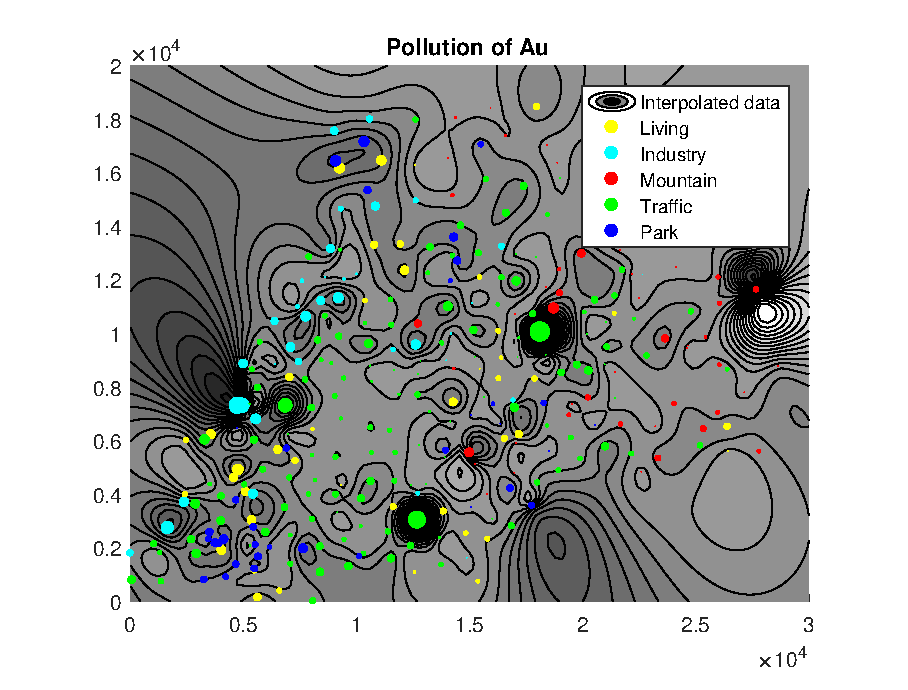
\includegraphics[scale=0.4]{pictures/pollution-of-Au.eps}
    \end{minipage}
    \begin{minipage}[t]{0.5\linewidth}
    \centering 
	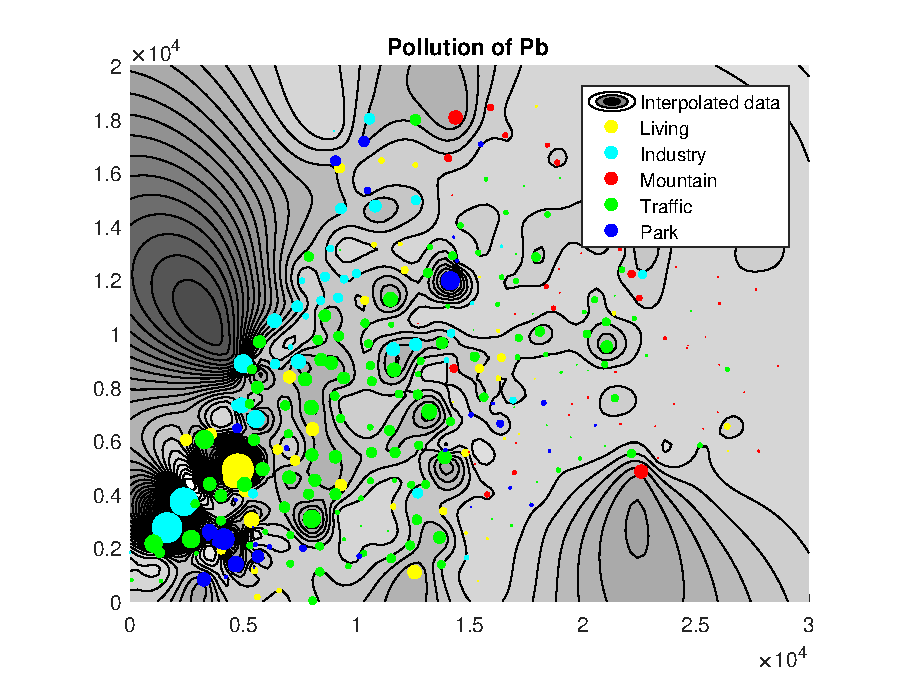
\includegraphics[scale=0.4]{pictures/pollution-of-Pb.eps}
    \end{minipage}
    \label{fig:char}
\end{figure}
从图中能够可以看出:
(1)重金属的分布具有富集性,即重金属在某个区域的分布含量很高,而在其他地方则含量较低。
(2)可以看出As在工业区的分布比较集中,而Pb在交通区域的分布非常密集。
(3)通过对其他重金属元素的平面分布的分析,我们发现不同重金属的分布具有鲜明的特征。往往在某一个区的分布非常密集。
进一步的分析表明:重金属的富集状态实际上是与区域的功能划分息息相关。
比如As主要分布于工业区,这是因为As是一种十分重要化工原料,在工业生产中必不可少,从而在工业区土壤中As含量很高。

\section{重金属的海拔分布}
将海拔每 10 米分一段,假设在某段中共有m个采样点,第i个采样点的重金属j的实测含量为$C_{ij}$,则该段中重金属j的平均含量$W_j$为:
\begin{equation}
W_j=\frac{1}{m}\sum_{i=1}^m C_{ij}
\end{equation}
根据上式,利用采样所得数据分别计算出各种重金属在不同海拔的平均含量。为了排除不同金属元素原本在土壤中含量差异的影响,我们对不同金属做了标准化处理:
\begin{equation}
W_j^{\prime} = \frac{W_j - \nu_j}{\sigma_j}
\end{equation}•
其中$\nu_j$和$\sigma_j$分别为第j重金属在土壤中含量的平均值和标准差
结果如下表所示:
\begin{table}[H]
		\centering
		\caption{不同海拔重金属平均含量}
		\label{average-contend}
		\begin{tabular}{c|cccccccc}
			hight	  &          	As	&   Cd   &     Cr     &   Cu   &     Hg  &    Ni   &     Pb    &   Zn  \\
			\hline
			 0-10m     	&	 7.0714  &  381.23  &  86.288  &  120.46 &   444.88 &   21.147 &   87.784  &  305.11     \\
    			10-20m     	&	 5.8219  &  340.52  &  48.867  &  47.638 &   405.32 &   17.031 &   67.277  &   239.25    \\
   			20-30m    	&	 5.726   &  319.98  &  50.278  &  50.464 &   391.49 &    17.52 &   59.443  &  259.07     \\
    			30-40m     	&	 5.6783  &  316.32  &   57.28  &  54.567 &   645.86 &   16.609 &    67.79  &  164.09     \\
    			40-50m     	&	 6.6211  &  328.15  &  42.978  &  39.453 &   117.18 &   16.979 &    52.31  &  154.99     \\
    			50-60m      	&	 5.125   & 260.62   & 41.036   & 43.522  &   66.08  &  14.783  &  55.222   & 124.81      \\
    			60-70m     	&	 4.4469  &  190.19  &  38.328  &  21.978 &   33.826 &   13.102 &   39.961  &   101.6     \\
    			70-80m     	&	 4.7492  &  264.49  &  55.809  &  30.905 &   60.671 &   22.693 &   9.755  &  205.65     \\
    			80-90m     	&	 3.8433  &  129.42  &  37.658  &  15.522 &   45.657 &   15.437 &   36.007  &  72.842     \\
    			90-100m    	&	 4.686   & 180.75   & 31.781   & 16.278  &  24.822  &  12.979  &  32.405   & 71.958      \\
    			>=100m    	&	 3.3381  &  168.67  &  34.459  &  12.831 &   37.124 &   13.316 &   38.689  &  73.364     \\
		\end{tabular}
	\end{table}
由上面的数据可以看出,总的来说各种重金属元素的含量随着海拔的升高而降低。这可能是因为人类活动的区域主要在低海拔地区,高海拔区受人类的影响较小。
此外,还可以发现,在70~80m的海拔高度上,大部分的重金属元素含量都要高于附近的海拔高度地区。
这一海拔高度多为山区,重金属含量高可能是因为汽车尾气,工厂废气中所含的重金属随大气运动进入这一地区的土壤所致。
也有可能是因为这一地区有采矿场的缘故。

\section{不同区域重金属污染情况}


\begin{equation}
\frac{\partial \rho}{\partial t} = \kappa \Delta \rho + \tau \Delta u
\end{equation}

\end{document}